\documentclass[11pt,a4paper]{book}
\usepackage[utf8]{inputenc}
\usepackage[T1]{fontenc}

% Math symbols and environments
%
% These have to be imported before some later package to prevent some
% redefinition error.
\usepackage{amsmath}
\usepackage{amssymb}
\usepackage{amsthm}

% Useful extensions for math
\usepackage{mathtools}

% Redefine spacing for proofs
\usepackage{thmtools}
\declaretheoremstyle[
  spaceabove=-4pt,
  spacebelow=8pt,
  headfont=\normalfont\itshape,
  postheadspace=1em,
  qed=\qedsymbol
]{nospacing}
\declaretheorem[name={Proof},style=nospacing,unnumbered]{proof2}

\usepackage{graphicx}
\usepackage[margin=3cm]{geometry}
\usepackage{microtype}
\usepackage[hidelinks]{hyperref}
\usepackage[style=alphabetic]{biblatex}
\usepackage{fancyhdr}

% Define subfigures
\usepackage{subcaption}

% Define an appendix
\usepackage[titletoc]{appendix}

% Do not indent paragraphs
\usepackage{parskip}

% Syntax highlighting
\usepackage{minted}

% Set global minted options
\setminted{linenos, autogobble, frame=lines, framesep=2mm}

% Do not show red boxes around characters, that pygments did not recognize,
% e.g. greek symbols
\makeatletter
\expandafter\def\csname PYGdefault@tok@err\endcsname{\def\PYGdefault@bc##1{{\strut ##1}}}
\makeatother

% Define replacements for UTF-8 characters in source code
\usepackage{newunicodechar}
\newunicodechar{μ}{$\mu$}
\newunicodechar{Σ}{$\Sigma$}

\newtheorem{lemma}{Lemma}
\newtheorem*{corollary}{Corollary}

\DeclareMathOperator{\supp}{supp}

\newcommand{\ontopof}[2]{
  \begin{array}{c}
    #1,\\#2
  \end{array}
}

% Inline Julia
\newcommand{\injulia}[1]{\mintinline{julia}{#1}}

% Do not break inline equations
\relpenalty=10000
\binoppenalty=10000

\addbibresource{references.bib}

\begin{document}

\pagestyle{empty}

\frontmatter

% Hide page numbers in frontmatter
\pagenumbering{gobble}

\begin{titlepage}
  \begingroup
  \begin{center}
    
\includegraphics[width=120pt]{thesis/logo}\\

    \vspace{9em}

    {\Huge Computations with Arbitrarily Distributed Random Variables}\\
    \vspace{2em}
    {\large Bachelor's Thesis}\\
    \vfill
    \small{\emph{Author}}\\
    \vspace{0.3em}
    {\LARGE Marten Lienen}\\
    \vspace{6em}
    \begin{minipage}{0.4\textwidth}
      \begin{flushleft}
        \small{\emph{Supervised by}}\\
        \vspace{0.3em}
        {\large Prof. Dr. Stefan Harmeling}
      \end{flushleft}
    \end{minipage}
    \hfill
    \begin{minipage}{0.4\textwidth}
      \begin{flushright}
        \small{\emph{Co-reviewed by}}\\
        \vspace{0.3em}
        {\large Prof. Dr. Michael Leuschel}
      \end{flushright}
    \end{minipage}
    \\
    \vspace{4em}
    {\Large Heinrich-Heine-Universität Düsseldorf}\\
    \vspace{0.5em}
    {\large Computer Vision, Computer Graphics and Pattern Recognition}\\
    \vspace{1em}
    July 21, 2015
  \end{center}
  \endgroup
\end{titlepage}

\cleardoublepage

\chapter*{Acknowledgements}

Thanks to Andreas Troll and Dr. Georg Jansing from the institute of applied
mathematics at HHU for explaining to me, why Gauss-Hermite quadrature is
unstable, when applied to the product of two Gaussian distributed random
variables.

Thanks to Prof.~Dr.~Stefan Harmeling for the idea, help, feedback and the
ongoing affirmation, that there must be a way to make this work.

\tableofcontents

\cleardoublepage

\mainmatter
\pagestyle{fancy}

\chapter{Introduction}

In the age of machine learning statistics and random variables have caught the
attention of computer scientists and software engineers. They try to estimate
the variables' parameters and properties from observed data and compute the
distributions of dependent variables from there. In this thesis we tackle the
latter problem. Its complexity varies from instance to instance.

As a simple example you might be interested in the sum of two estimated random
variables, which you assume to be Gaussian distributed. The sum's distribution
can be worked out formally through basic analysis, which can even be done by
hand.
\begin{equation*}
  X \sim \mathcal{N}(\mu, \sigma) \qquad Y \sim \mathcal{N}(\nu, \tau) \qquad \Rightarrow \qquad Z = X + Y \sim \mathcal{N}(\mu + \nu, \sigma + \tau)
\end{equation*}

Most cases however are not manageable without the assistance of computing
software like Maple \cite{maple}. The following Maple program computes the
probability density function (PDF) of the quotient of two random variables as
defined in the previous paragraph. A quick look at figure
\ref{fig:intro-maple-pdf} should tell you, that you probably would not stand a
chance with pen and paper.
\begin{minted}{python}
  with(Statistics);
  X := RandomVariable(Normal(mu, sigma));
  Y := RandomVariable(Normal(nu, tau));
  Z := X/Y;
  PDF(Z, z);
\end{minted}
\begin{figure}
  \begin{subfigure}{0.45\textwidth}
    \centering
    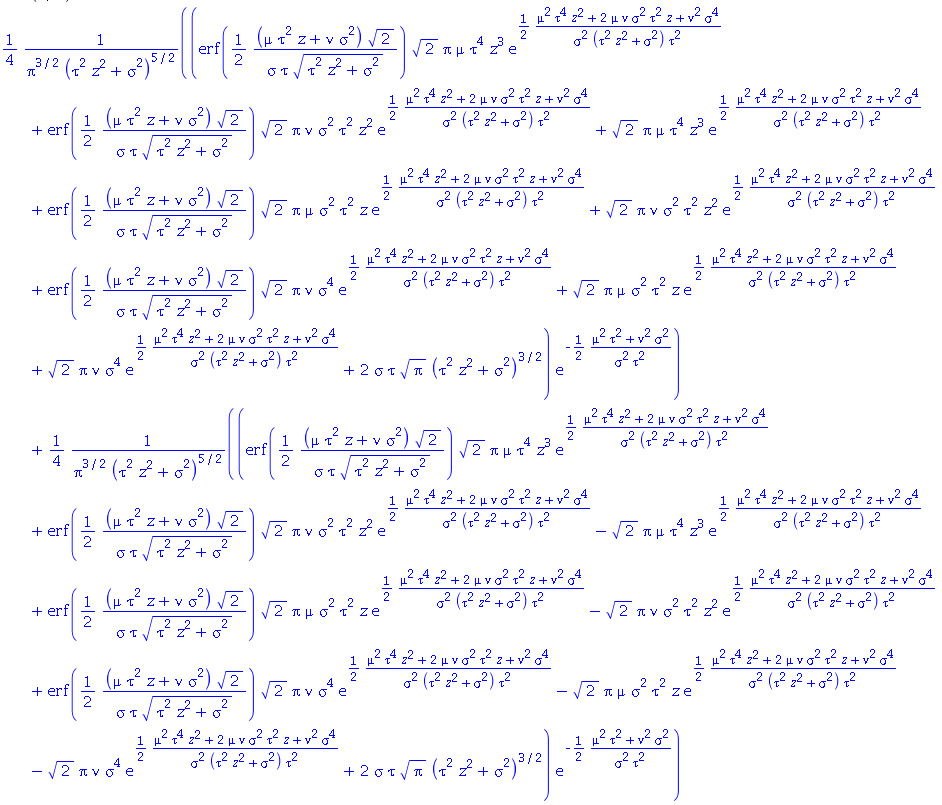
\includegraphics[width=\textwidth]{thesis/introduction/maple-pdf}
    \caption{Symbolic PDF}
  \end{subfigure}
  \hfill
  \begin{subfigure}{0.45\textwidth}
    \centering
    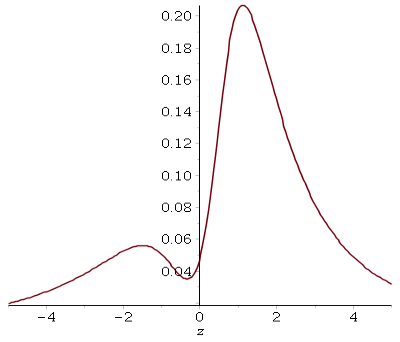
\includegraphics[width=\textwidth]{thesis/introduction/maple-plot}
    \caption{Plot for $\mu = 2, \nu = 0.5, \sigma = \tau = 1$}
  \end{subfigure}
  \caption{Maple finds a symbolic representation of the result's distribution}
  \label{fig:intro-maple-pdf}
\end{figure}

The approach of ramping up computing power and letting the computer find a
symbolic solution also has its limitations though. If you combine enough random
variables with different operations, a technical computing solution will either
be unable to find a solution or the found solution will contain so many
left-over integrals and costly functions, that actually evaluating it is not
feasible. At this point you have to resort to sampling. This means, that you
sample $n$ times from your random variables and compute $n$ samples of the
dependent variable. You can then use sample statistics to estimate basic
properties of the dependent variable and a histogram of the samples is an
approximation to its PDF. The probabilistic programming community \cite{ppl} has
developed various libraries and whole programming languages to explore sampling
techniques. The next program is written in one of these called Church
\cite{church}. It samples from three random variables with different
distributions and computes samples of the dependent variable from them. We
obtain the approximation in figure \ref{fig:church-pdf}, even when Maple was not
able to handle this at all and just reported $\infty$.
\begin{minted}{scheme}
  (define (sample)
    (define x1 (gaussian 1 2))
    (define x2 (gamma 1 3))
    (define y (exponential 2))

    (/ (* x1 x2) y))

  (define samples (repeat 100000 sample))
\end{minted}
\begin{figure}[h]
  \centering
  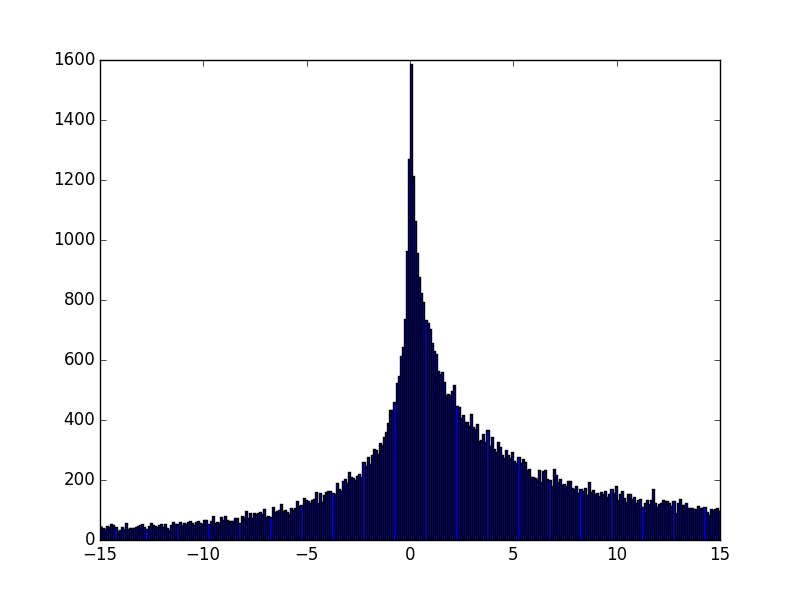
\includegraphics[width=300px]{thesis/introduction/church-pdf}
  \caption{Approximation to a complicated PDF obtained by sampling}
  \label{fig:church-pdf}
\end{figure}

Symbolic representations give you a way to handle exact solutions in a compact
form. The downside is, that they are restricted to simple problems and the
resulting formulas can be very complicated and expensive to evaluate. Sampling
can cope with every combination, that is computable, but is only
approximate. Our approach lies between symbolic representation and sampling, a
symbolic approximation. We find a symbolic representation that can approximate
arbitrary probability distributions and at the same time is closed under certain
operations. So you can do calculations with distributions of your choosing and
still obtain a symbolic result.

We will
\begin{itemize}
\item formalize the problem and explain our idea in detail (Section
  \ref{ch:idea})
\item describe a way to represent any distribution as a mixture of Gaussians
  (Section \ref{sec:em})
\item prove, that mixture distributions are closed under certain operations and
  are thus a good fit as a mathematical framework (Section \ref{sec:closure})
\item explore the viability of Gaussians as component distributions (Section
  \ref{sec:gaussians})
\item describe the structure of the julia implementation (Section
  \ref{ch:implementation})
\item showcase our results and compare them to ones that were derived
  symbolically or through sampling (Section \ref{ch:comparisons})
\item conclude this thesis with ideas for further work (Section
  \ref{ch:conclusions})
\end{itemize}

\chapter{Our Approach}
\label{ch:idea}

Consider $X_{i} \in \mathbb{R}, i \in \{ 1, \dots, n \}$ $n$ independent random
variables with known PDFs $p(X_{i}\hspace{0.1em}=\hspace{0.1em}x)$,
$f : \bigtimes_{i} \supp(X_{i}) \rightarrow \mathbb{R}$ a function defined on at
least the support of all the $X_{i}$ and $Y = f(X_{1}, \dots, X_{n})$ the
dependent variable. The task is then to derive the probability distribution of
$Y$ or at least an approximation to it from the known distributions of the
$X_{i}$.

As explained in the first chapter, this problem is very hard in its full
generality. Therefore we are going to simplify it by restricting the $X_{i}$ as
well as $f$. First, we restrict the distributions of the $X_{i}$ to mixture
distributions, especially mixtures of Gaussians. The first advantage of mixtures
of Gaussians is, that with enough components you can approximate any
distribution to arbitrary precision as you can see in figure
\ref{fig:idea-em}. So we have simplified one aspect of the problem, while still
being able to model any distribution. The other advantage is, that Gaussian
distributions are closed under addition and subtraction and the products and
quotients can be closely approximated by mixtures of Gaussians. This is
important, because these closure properties of distributions are preserved, when
you consider a mixture of them, as we see in section \ref{sec:closure}.
\begin{figure}[h]
  \centering
  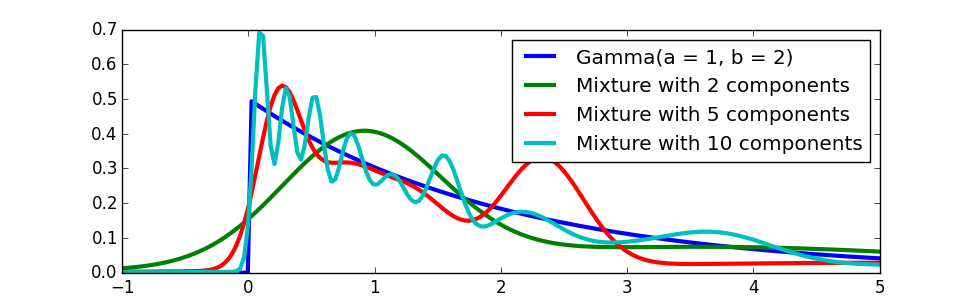
\includegraphics[width=0.8\textwidth]{thesis/idea/em}
  \caption{A gamma distribution approximated by mixtures of Gaussians}
  \label{fig:idea-em}
\end{figure}

Secondly, we only consider $f$, that are differentiable and invertible in the
first argument. The reasoning is that for such $f$ there is a lemma called
\emph{multivariate change of variables} \cite[chapter~2.6.2.1]{murphy}, that
lets you reduce the distribution of $Y$ to the joint distribution of the
$X_{i}$. This in turn lets us prove, that the family of mixture distributions is
closed under any such $f$ (section \ref{sec:closure}).

With these restrictions in place we can give symbolic approximations for any $Y$
as long as Gaussian distributions are closed under $f$ or the result of $f$ can
at least be reasonably well approximated by a mixture of Gaussians.

\chapter{The Details}
\label{ch:theory}

In this chapter we will work out the details. We begin with explaining how to
convert arbitrary distributions into mixtures of Gaussians. Then we will prove,
that mixture distributions are closed under certain functions. In the end we
will look at Gaussians as component distributions of mixture distributions and
give exact results and approximations for basic function applications.

\section{Modelling Distributions as Mixtures of Gaussians}
\label{sec:em}

The first step is based on the expectation-maximization (EM) algorithm
\cite[chapter~11.4.2]{murphy}, an iterative algorithm to fit a mixture of
Gaussians to best explain a set of samples. To find a mixture of Gaussians, that
models a given distribution $p$, you first draw a set of samples from $p$. These
samples are obviously distributed according to $p$, so when you fit a mixture of
Gaussians with EM to best explain them, i.e. maximize the likelihood, it will
closely model $p$.

\begin{figure}[h]
  \centering
  \begin{subfigure}{0.45\textwidth}
    \centering
    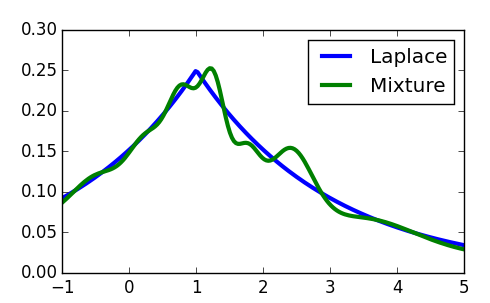
\includegraphics[width=\textwidth]{thesis/theory/em-laplace}
    \caption{A Laplace distribution with $a = 1, b = 2$}
  \end{subfigure}
  \hfill
  \begin{subfigure}{0.45\textwidth}
    \centering
    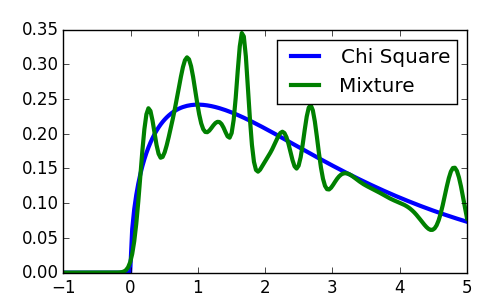
\includegraphics[width=\textwidth]{thesis/theory/em-chisq}
    \caption{A chi-squared distribution with $k = 3$}
  \end{subfigure}
  \caption{Some distributions modelled as mixtures of Gaussians}
  \label{fig:theory-em}
\end{figure}

As shown in figure \ref{fig:theory-em} EM also works for distributions, that do
not share many properties with Gaussians, but yields the best results for
distributions that have whole $\mathbb{R}$ as support.

\section{Closure of Mixtures}
\label{sec:closure}

Let $X$ and $Y_{1}, \dots, Y_{n}$ be random variables with mixture distribution,
i.e.
\begin{equation*}
  p(X = x) = \sum_{i = 1}^{m} \alpha_{i} \cdot p(X_{i} = x) \qquad p(Y_{i} = y) = \sum_{j = 1}^{m_{i}} \beta_{i,j} \cdot p(Y_{i,j} = y)
\end{equation*}
where the $X_{i}$ and $Y_{i, j}$ are random variables distributed like the
component distributions of $X$ respectively $Y_{i}$.

Consider a function $f : S \times_{i = 1}^{n} S_{i} \rightarrow \mathbb{R}$,
where $S \supseteq \supp(X)$ and
$S_{i} \supseteq \supp(Y_{i}), i \in \{ 1, \dots, n \}$. Then we might ask
ourselves, how $Z = f(X, Y_{1}, \dots, Y_{n})$ is distributed. So we are looking
to evaluate
\begin{equation*}
  p(Z = z) = \int_{S_{n}}\dots\int_{S_{1}} p(Z = 1, Y_{1} = y_{1}, \dots, Y_{n} = y_{n})~\mathrm{d}y_{1}\dots\mathrm{d}y_{n}
\end{equation*}

First, we have to tie the joint PDF of $Z$ and $Y_{1, \dots, n}$ to the joint
PDF of $X$ and $Y_{1, \dots, n}$. Such an expression can be derived using
\emph{multivariate change of variables} \cite[chapter~2.6.2.1]{murphy}, which I
will restate here.

\begin{lemma}[Multivariate change of variables]
  \label{lemma:multivariate-change}
  Let $f : \mathbb{R}^{n} \rightarrow \mathbb{R}^{n}$ be differentiable and
  invertible, $X \in \mathbb{R}^{n}$ a random vector and $Y = f(X)$. Then the
  distribution of $Y$ is given by
  \begin{equation*}
    p(Y = y) = \left| \det J \right| \cdot p(X = f^{-1}(y))
  \end{equation*}
  where $J$ is the Jacobian of $f^{-1}$, i.e.
  \begin{equation*}
    J = \frac{\partial X}{\partial Y} = \begin{pmatrix}
      \frac{\partial X_{1}}{\partial Y_{1}} & \cdots & \frac{\partial X_{1}}{\partial Y_{n}}\\
      \vdots & \ddots & \vdots\\
      \frac{\partial X_{n}}{\partial Y_{1}} & \cdots & \frac{\partial X_{n}}{\partial Y_{n}}
    \end{pmatrix}
  \end{equation*}
\end{lemma}

For the rest of this section we will use $p(Y_{1, \dots, n} = y_{1, \dots, n})$
as a shorthand for $p(Y_{1} = y_{1}, \dots, Y_{n} = y_{n})$. Also
$f^{-1}_{y_{1}, \dots, y_{n}}$ should be read as the inverse of $f$ in the first
argument with $y_{1}, \dots, y_{n}$ held constant, i.e.
\begin{equation*}
  f^{-1}_{y_{1}, \dots, y_{n}}(f(z, y_{1}, \dots, y_{n})) = z
\end{equation*}

\begin{lemma}
  \label{lemma:joint-pdf}
  If $f$ is differentiable and invertible in the first argument, we can express
  the joint PDF of $Z$ and $Y_{1, \dots, n}$ in terms of the joint PDF of $X$
  and $Y_{1, \dots, n}$ as
  \begin{equation*}
    p(Z = z, Y_{1, \dots, n} = y_{1, \dots, n}) = \left| \frac{\mathrm{d}f_{y_{1}, \dots, y_{n}}^{-1}(z)}{\mathrm{d}z} \right| \cdot p\left(X = f_{y_{1}, \dots, y_{n}}^{-1}(z), Y_{1, \dots, n} = y_{1, \dots, n}\right)
  \end{equation*}
\end{lemma}
\begin{proof2}
  Define $g : S \times_{i = 1}^{n} S_{i} \rightarrow \mathbb{R}^{n + 1}$ as
  \begin{equation*}
    g \begin{pmatrix}
      x\\y_{1}\\\vdots\\y_{n}
    \end{pmatrix} = \begin{pmatrix}
      f(x, y_{1}, \dots, y_{n})\\
      y_{1}\\\vdots\\y_{n}
    \end{pmatrix}
  \end{equation*}
  Then $g$ is invertible and differentiable and the inverse is given by
  \begin{equation*}
    g^{-1}\begin{pmatrix}
      z\\y_{1}\\\vdots\\y_{n}
    \end{pmatrix} = \begin{pmatrix}
      f_{y_{1}, \dots, y_{n}}^{-1}(z)\\
      y_{1}\\\vdots\\y_{n}
    \end{pmatrix}
  \end{equation*}
  Next we examine the Jacobian $J$ of $g^{-1}$. Let
  $(z, y_{1}, \dots, y_{n})^{T} \in \mathbb{R}^{n + 1}$.
  \begin{equation*}
    J =
    \begin{pmatrix}
      \frac{\mathrm{d}f_{y_{1}, \dots, y_{n}}^{-1}}{\partial z} & \frac{\mathrm{d}f_{y_{1}, \dots, y_{n}}^{-1}}{\partial y_{1}} & \cdots & \frac{\mathrm{d}f_{y_{1}, \dots, y_{n}}^{-1}}{\partial y_{n}}\\
      \frac{\mathrm{d} y_{1}}{\mathrm{d} z} & \frac{\mathrm{d} y_{1}}{\mathrm{d} y_{1}} & \cdots & \frac{\mathrm{d} y_{1}}{\mathrm{d} y_{n}}\\
      \vdots & \vdots & \ddots & \vdots\\
      \frac{\mathrm{d} y_{n}}{\mathrm{d} z} & \frac{\mathrm{d} y_{n}}{\mathrm{d} y_{1}} & \cdots & \frac{\mathrm{d} y_{n}}{\mathrm{d} y_{n}}
    \end{pmatrix}
    =
    \begin{pmatrix}
      \frac{\mathrm{d}f_{y_{1}, \dots, y_{n}}^{-1}}{\partial z} & \frac{\mathrm{d}f_{y_{1}, \dots, y_{n}}^{-1}}{\partial y_{1}} & \cdots & \frac{\mathrm{d}f_{y_{1}, \dots, y_{n}}^{-1}}{\partial y_{n}}\\
      0 & 1 & \cdots & 0\\
      \vdots & \vdots & \ddots & \vdots\\
      0 & 0 & \cdots & 1
    \end{pmatrix}
  \end{equation*}
  $J$ is an upper-triangular matrix, which means
  \begin{equation*}
    \det J = \frac{\mathrm{d}f_{y_{1}, \dots, y_{n}}^{-1}}{\partial z}
  \end{equation*}
  Therefore the claimed equality follows from lemma \ref{lemma:multivariate-change}.
\end{proof2}

Equipped with lemma \ref{lemma:joint-pdf} we can now derive the general form of
$Z$'s distribution.

\begin{lemma}
  \label{lemma:mixture}
  If $f$ is differentiable and invertible in the first argument, the
  distribution of $Z$ is a mixture distribution given by the following equation
  \begin{equation*}
    p(Z = z) = \sum_{i = 1}^{m} \sum_{k_{1} = 1}^{m_{1}} \dots \sum_{k_{n} = 1}^{m_{n}} \alpha_{i} \left( \prod_{j = 1}^{n} \beta_{j,k_{j}} \right) p(f(X_{i}, Y_{1,k_{1}}, \dots, Y_{n,k_{n}}) = z)
  \end{equation*}
\end{lemma}
\begin{proof2}
  \begin{align*}
    \intertext{Expand marginal distribution as an integral over the joint distribution}
    & p(Z = z) = \int_{S_{n}} \dots \int_{S_{1}} p(Z = z, Y_{1, \dots, n} = y_{1, \dots, n})~\mathrm{d}y_{1}\dots \mathrm{d}y_{n}\\
    \intertext{Rewrite it using lemma \ref{lemma:joint-pdf}}
    = & \int_{S_{n}} \dots \int_{S_{1}} \left| \frac{\mathrm{d}x}{\mathrm{d}z} \right| \cdot p\left(X = f_{y_{1}, \dots, y_{n}}^{-1}(z), Y_{1, \dots, n} = y_{1, \dots, n}\right)~\mathrm{d}y_{1}\dots \mathrm{d}y_{n}\\
    \intertext{Use the fact, that $X$ and $Y_{i}$ are independent, i.e. that the joint PDF can be factorized}
    = & \int_{S_{n}} \dots \int_{S_{1}} \left| \frac{\mathrm{d}x}{\mathrm{d}z} \right| \cdot p\left(X = f_{y_{1}, \dots, y_{n}}^{-1}(z)\right) \prod_{j = 1}^{n} p\left(Y_{j} = y_{j}\right)~\mathrm{d}y_{1}\dots \mathrm{d}y_{n}\\
    \intertext{Plug in the distributions of $X$ and $Y_{i}$}
    = & \int_{S_{n}} \dots \int_{S_{1}} \left| \frac{\mathrm{d}x}{\mathrm{d}z} \right| \cdot \left(\sum_{i = 1}^{m} \alpha_{i} \cdot p(X_{i} = f_{y_{1}, \dots, y_{n}}^{-1}(z))\right) \prod_{j = 1}^{n} \left(\sum_{k = 1}^{m_{j}} \beta_{j,k} \cdot p(Y_{j,k} = y_{j})\right)~\mathrm{d}y_{1}\dots \mathrm{d}y_{n}\\
    \intertext{Pull out the coefficients}
    = & \sum_{i = 1}^{m} \sum_{k_{1} = 1}^{m_{1}} \dots \sum_{k_{n} = 1}^{m_{n}} \alpha_{i} \left( \prod_{j = 1}^{n} \beta_{j,k_{j}} \right) \int\limits_{S_{n}} \dots \int\limits_{S_{1}} \left| \frac{\mathrm{d}x}{\mathrm{d}z} \right| \cdot p(X_{i} = f_{y_{1}, \dots, y_{n}}^{-1}(z)) \cdot \prod_{j = 1}^{n} p(Y_{j,k_{j}} = y_{j})~\mathrm{d}y_{1}\dots \mathrm{d}y_{n}\\
    \intertext{Join the probability densities together}
    = & \sum_{i = 1}^{m} \sum_{k_{1} = 1}^{m_{1}} \dots \sum_{k_{n} = 1}^{m_{n}} \alpha_{i} \left( \prod_{j = 1}^{n} \beta_{j,k_{j}} \right) \int\limits_{S_{n}} \dots \int\limits_{S_{1}} \left| \frac{\mathrm{d}x}{\mathrm{d}z} \right| \cdot p\left( \ontopof{X_{i} = f_{y_{1}, \dots, y_{n}}^{-1}(z)}{Y_{1,k_{1}} = y_{1}, \dots, Y_{n,k_{n}} = y_{n}} \right)~\mathrm{d}y_{1}\dots \mathrm{d}y_{n}\\
    \intertext{Reverse application of lemma \ref{lemma:joint-pdf}}
    = & \sum_{i = 1}^{m} \sum_{k_{1} = 1}^{m_{1}} \dots \sum_{k_{n} = 1}^{m_{n}} \alpha_{i} \left( \prod_{j = 1}^{n} \beta_{j,k_{j}} \right) \int\limits_{S_{n}} \dots \int\limits_{S_{1}} p\left( \ontopof{f(X_{i}, Y_{1,k_{1}}, \dots, Y_{n,k_{n}}) = z}{Y_{1,k_{1}} = y_{1}, \dots, Y_{n,k_{n}} = y_{n}} \right)~\mathrm{d}y_{1}\dots \mathrm{d}y_{n}\\
    \intertext{Marginalize the $Y_{i}$}
    = & \sum_{i = 1}^{m} \sum_{k_{1} = 1}^{m_{1}} \dots \sum_{k_{n} = 1}^{m_{n}} \alpha_{i} \left( \prod_{j = 1}^{n} \beta_{j,k_{j}} \right) p(f(X_{i}, Y_{1,k_{1}}, \dots, Y_{n,k_{n}}) = z)
  \end{align*}
\end{proof2}

\begin{lemma}
  \label{lemma:components}
  If $f(X_{i}, Y_{1,k_{1}}, \dots, Y_{n,k_{n}})$ has a mixture distribution, $Z$
  has a mixture distribution as well.
\end{lemma}
\begin{proof2}
  We will not proof it in full rigor, because it is only one rearrangement, but
  would involve a lot of additional indices for the distribution of $f$.
  \begin{align*}
    p(Z = z) = & \sum_{i = 1}^{m} \sum_{k_{1} = 1}^{m_{1}} \dots \sum_{k_{n} = 1}^{m_{n}} \alpha_{i} \left( \prod_{j = 1}^{n} \beta_{j,k_{j}} \right) p(f(X_{i}, Y_{1,k_{1}}, \dots, Y_{n,k_{n}}) = z)\\
    \intertext{Plug in the mixture distribution of $f$}
    = & \sum_{i = 1}^{m} \sum_{k_{1} = 1}^{m_{1}} \dots \sum_{k_{n} = 1}^{m_{n}} \alpha_{i} \left( \prod_{j = 1}^{n} \beta_{j,k_{j}} \right) \sum_{p} \gamma_{p} p_{f}(z)\\
    \intertext{Push the coefficients of $Z$ into the inner sum}
    = & \sum_{i = 1}^{m} \sum_{k_{1} = 1}^{m_{1}} \dots \sum_{k_{n} = 1}^{m_{n}} \sum_{p} \alpha_{i} \left( \prod_{j = 1}^{n} \beta_{j,k_{j}} \right) \gamma_{p} p_{f}(z)\\
  \end{align*}
\end{proof2}

Lemma \ref{lemma:mixture} and \ref{lemma:components} together are the foundation
of this thesis. They say, that if $X$ and the $Y_{i}$ have a mixture of $P$
(e.g. Gaussians) distribution, $Z$ will have a mixture of $P$ distribution as
well, if $f$ applied to the component distributions of $X$ and $Y_{i}$ is
distributed as $P$ or a mixture of $P$. This means, that to prove results in our
restricted setting, we only need to prove it for $P$-distributed variables and
it will generalize to mixtures of $P$ automatically.

\section{Gaussians as Component Distributions}
\label{sec:gaussians}

In this section we focus on Gaussian distributions and how to express the
distributions of basic $f(X_{1}, \dots, X_{n})$ as mixtures of gaussians.

\subsection{Affine Transformations}
\label{sec:affine-transforms}

Let $X$ be a random variable with a Gaussian distribution, i.e.
$X \sim \mathcal{N}(\mu, \sigma^{2})$. A basic thing to do with $X$ is to apply
an affine transformation, because every operation involved is just a
transformation of the parameters of the original distribution, as we will
presently see. Along the way we will also reduce subtraction and division to
addition respectively multiplication, because they enhance the usability of the
julia library.

First we need to establish two rearrangement rules for Gaussian distributions.
\begin{lemma}
  \label{lemma:x-mu-symmetry}
  Let $a \in \mathbb{R}$. Then
  $\mathcal{N}(x + a \mid \mu, \sigma^{2}) = \mathcal{N}(x \mid \mu - a,
  \sigma^{2})$.
\end{lemma}
\begin{proof2}
  \begin{align*}
    \mathcal{N}(x + a \mid \mu, \sigma^{2}) = & \frac{1}{\sqrt{2 \pi \sigma^{2}}} \exp\left( - \frac{\left((x + a) - \mu \right)^{2}}{2\sigma^{2}} \right)\\
    = & \frac{1}{\sqrt{2 \pi \sigma^{2}}} \exp\left( - \frac{\left(x - (\mu - a) \right)^{2}}{2\sigma^{2}} \right) = \mathcal{N}(x \mid \mu - a, \sigma^{2})
  \end{align*}
\end{proof2}

\begin{lemma}
  \label{lemma:gaussian-parameter-scaling}
  Let $a \in \mathbb{R} \setminus \{ 0 \}$. Then
  $\mathcal{N}(ax \mid \mu, \sigma^{2}) = \frac{1}{|a|} \cdot \mathcal{N}\left(x \mid
  \frac{\mu}{a}, \frac{\sigma^{2}}{a^{2}}\right)$.
\end{lemma}
\begin{proof2}
  \begin{align*}
    \mathcal{N}(ax \mid \mu, \sigma^{2}) = & \frac{1}{\sqrt{2 \pi \sigma^{2}}} \exp\left( -\frac{\left(ax - \mu \right)^{2}}{2\sigma^{2}} \right)\\
    = & \frac{1}{\sqrt{2 \pi \left( \frac{\sigma a}{a} \right)^{2}}} \exp\left( -\frac{a^{2}\left(x - \frac{\mu}{a} \right)^{2}}{2\sigma^{2}} \right)\\
    = & \frac{1}{|a|} \frac{1}{\sqrt{2 \pi \frac{\sigma^{2}}{a^{2}}}} \exp\left( -\frac{\left(x - \frac{\mu}{a} \right)^{2}}{2 \frac{\sigma^{2}}{a^{2}}} \right)\\
    = & \frac{1}{|a|} \cdot \mathcal{N}\left( x \mid \frac{\mu}{a}, \frac{\sigma^{2}}{a^{2}} \right)
  \end{align*}
\end{proof2}

Next we restate a special case of lemma \ref{lemma:multivariate-change} taken
from \cite[chapter~2.6.2]{murphy}.
\begin{lemma}[Change of variables]
  \label{lemma:change}
  Let $f : \mathbb{R} \rightarrow \mathbb{R}$ be differentiable, monotonic and
  hence invertible. We can ``unapply'' $f$ through the following formula
  \begin{equation*}
    p(f(X) = y) = \left| \frac{\mathrm{d}f^{-1}}{\mathrm{d}y} \right| \cdot p(X = f^{-1}(y))
  \end{equation*}
\end{lemma}

With these in place we can now examine addition, subtraction, multiplication and
division with a scalar.

\vspace{1em}

\begin{lemma}
  $-X \sim \mathcal{N}(-\mu, \sigma^{2})$
\end{lemma}
\begin{proof2}
  This follows directly from lemma \ref{lemma:gaussian-parameter-scaling} and
  \ref{lemma:change}.
  \begin{equation*}
    p(-X = x) = \mathcal{N}((-1)x \mid \mu, \sigma^{2}) = \frac{1}{|{-1}|} \cdot \mathcal{N}\left( x \mid \frac{\mu}{{-1}}, \frac{\sigma^{2}}{({-1})^{2}} \right) = \mathcal{N}(x \mid {-\mu}, \sigma^{2})
  \end{equation*}
\end{proof2}

\begin{lemma}
  Let $a \in \mathbb{R}$. Then
  $a + X = X + a \sim \mathcal{N}(\mu + a, \sigma^{2})$.
\end{lemma}
\begin{proof2}
  This follows directly from lemma \ref{lemma:x-mu-symmetry} and
  \ref{lemma:change}.
  \begin{align*}
    p(X + a = x) = p(X = x - a) \cdot \left| \frac{\mathrm{d}(x - a)}{\mathrm{d}x} \right| = \mathcal{N}(x - a \mid \mu, \sigma^{2}) = \mathcal{N}(x \mid \mu + a, \sigma^{2})
  \end{align*}
\end{proof2}

\begin{corollary}
  Let $a \in \mathbb{R}$. Then $X - a \sim \mathcal{N}(\mu - a, \sigma^{2})$.
\end{corollary}
\begin{proof2}
  $X - a = X + (-a)$
\end{proof2}

\begin{corollary}
  Let $a \in \mathbb{R}$. Then $a - X \sim \mathcal{N}(a - \mu, \sigma^{2})$.
\end{corollary}
\begin{proof2}
  $a - X = a + (-X)$
\end{proof2}

\begin{lemma}
  Let $a \in \mathbb{R} \setminus \{ 0 \}$. Then
  $aX = Xa \sim \mathcal{N}(a\mu, a^{2}\sigma^{2})$.
\end{lemma}
\begin{proof2}
  This follows from lemma \ref{lemma:gaussian-parameter-scaling} and
  \ref{lemma:change}.
  \begin{align*}
    p(aX = x) & = \left| \frac{\mathrm{d}\frac{x}{a}}{\mathrm{d}x} \right| \cdot p\left( X = \frac{x}{a} \right)\\
              & = \left|\frac{1}{a}\right| \cdot p\left( X = \frac{x}{a} \right)\\
              & = \left|\frac{1}{a}\right| \cdot \mathcal{N}\left(\frac{x}{a} \mid \mu, \sigma^{2}\right)\\
              & = \frac{1}{|a|} \cdot |a| \cdot \mathcal{N}\left(x \mid a\mu, a^{2}\sigma^{2}\right)\\
              & = \mathcal{N}\left(x \mid a\mu, a^{2}\sigma^{2}\right)
  \end{align*}
\end{proof2}

\begin{corollary}
  Let $a \in \mathbb{R} \setminus \{ 0 \}$. Then
  $\frac{X}{a} \sim \mathcal{N}\left( \frac{\mu}{a}, \frac{\sigma^{2}}{a^{2}}
  \right)$.
\end{corollary}
\begin{proof2}
  $\frac{X}{a} = X \cdot \frac{1}{a}$
\end{proof2}

Note, that we did not cover $\frac{a}{X}$. Division is not monotonic for a
variable denominator, so lemma \ref{lemma:change} does not hold and the
distribution of $\frac{a}{X}$ cannot be evaluated with the techniques used in
this section.

\subsection{Affine Transformations of $n$ Variables}

A natural enhancement of section \ref{sec:affine-transforms} is to generalize it
to multiple variables. Therefore we will first determine the distribution of the
sum of two Gaussian distributed variables.

\begin{lemma}
  \label{lemma:gaussian-sum}
  Let $X \sim \mathcal{N}(\mu, \sigma^{2}), Y \sim \mathcal{N}(\nu, \tau^{2})$
  be two independent, Gaussian distributed variables. The distribution of their
  sum is
  \begin{equation*}
    X + Y \sim \mathcal{N}(\mu + \nu, \sigma^{2} + \tau^{2})
  \end{equation*}
\end{lemma}
\begin{proof2}
  For a proof see \cite[Satz~11.9]{krengel}.
\end{proof2}

With lemma \ref{lemma:gaussian-sum} combined with the previous section, we can
now calculate the distribution of a linear combination of two Gaussian
distributed variables. Applying this inductively, we can evaluate affine
transformations of $n$ variables.

\subsection{Products of Gaussian Random Variables}

Multiplication is indeed monotonic and invertible in the first argument, but
differs from the previous operations in that Gaussian distributions are not
closed under it. Actually the products of two gaussians do not have any standard
distribution at all. So to stay inside the realm of mixtures of Gaussians, we
have to approximate them with a mixture of Gaussians using numerical integration
algorithms.

Let $X$ and $Y$ be two normally distributed variables
\begin{equation*}
  X \sim \mathcal{N}(\mu, \sigma^{2}) \qquad Y \sim \mathcal{N}(\nu, \tau^{2})
\end{equation*}
and $Z = X \cdot Y$ their product. Then $Z$ is distributed as follows
\begin{align*}
  p(Z = z) & = \int_{-\infty}^{\infty} \frac{1}{|y|} \cdot p\left(X = \frac{z}{y}\right) \cdot p(Y = y)~\mathrm{d}y\\
           & = \int_{-\infty}^{\infty} \frac{1}{|y|} \cdot \mathcal{N}\left( \frac{z}{y} \mid \mu, \sigma^{2} \right) \cdot \mathcal{N}(y \mid \nu, \tau^{2})~\mathrm{d}y\\
           & = \int_{-\infty}^{\infty} \frac{1}{|y|} \cdot |y| \cdot \mathcal{N}\left( z \mid y\mu, y^{2}\sigma^{2} \right) \cdot \mathcal{N}(y \mid \nu, \tau^{2})~\mathrm{d}y\\
           & = \int_{-\infty}^{\infty} \mathcal{N}\left( z \mid y\mu, y^{2}\sigma^{2} \right) \cdot \mathcal{N}(y \mid \nu, \tau^{2})~\mathrm{d}y
\end{align*}

We would like to write this as a mixture of Gaussians, i.e.
$\sum_{i} \alpha_{i} \cdot \mathcal{N}(\mu_{i}, \sigma_{i})$. Gaussian
quadrature comes to mind, a family of numerical integration algorithms, that
approximate
\begin{equation*}
  \int_{a}^{b} f(x) \cdot w(x)~\mathrm{d}x \approx \sum_{i = 1}^{n} w_{i} f(x_{i})
\end{equation*}
with $n$ summands for various combinations of $a$, $b$ and $w$ as long as the
integrand can be written as $f(x) \cdot w(x)$, where $w$ is a weight function
determined by the specific algorithm and $f$ an arbitrary function from
$C^{2n - 1}[a, b]$. $C^{n}[a, b]$ is thereby defined as the set of all
functions, that are at least $n$ times continuously differentiable on $[a, b]$.
It probably does not need to be mentioned, but the approximation becomes more
accurate with increasing $n$.

\subsubsection{Gauss-Hermite Quadrature}

Gauss-Hermite quadrature is a special case of Gauss quadrature for integrals of
the form
\begin{equation*}
  \int_{-\infty}^{\infty} f(x) \cdot \exp(-x^{2})~\mathrm{d}x
\end{equation*}
This looks like a perfect fit for our integral, because the PDF of a Gaussian
distribution is practically of the form $a \cdot \exp(-x^{2})$, so one of the
Gaussians can serve as the weight function, while the other persists as part of
$f$ creates the Gaussians in the resulting mixture of Gaussians.

\begin{align*}
  p(Z = z) & = \int_{-\infty}^{\infty} \mathcal{N}\left( z \mid y\mu, y^{2}\sigma^{2} \right) \cdot \mathcal{N}(y \mid \nu, \tau^{2})~\mathrm{d}y\\
           & = \int_{-\infty}^{\infty} \mathcal{N}\left( z \mid y\mu, y^{2}\sigma^{2} \right) \cdot \frac{1}{\sqrt{2\pi\tau^{2}}} \exp\left( -\frac{(y - \nu)^{2}}{2\tau^{2}} \right)~\mathrm{d}y\\
  \intertext{To transform the integrand into the form $f(x) \cdot \exp(-x^{2})$ we will now substitute
\begin{equation*}
  x = \frac{y - \nu}{\sqrt{2}\tau} \Leftrightarrow y = \sqrt{2}\tau x + \nu \qquad \frac{\mathrm{d}x}{\mathrm{d}y} = \frac{1}{\sqrt{2}\tau}
\end{equation*}}
           & = \frac{1}{\sqrt{\pi}} \int_{-\infty}^{\infty} \mathcal{N}\left( z \mid \left(\sqrt{2}\tau x + \nu\right)\mu, \left(\sqrt{2}\tau x + \nu\right)^{2}\sigma^{2} \right) \cdot \exp\left( -x^{2} \right)~\mathrm{d}x
\end{align*}

With the integrand in the right form we can apply the approximation.
\begin{equation*}
  p(Z = z) \approx \sum_{i = 1}^{n} \frac{w_{i}}{\sqrt{\pi}} \cdot \mathcal{N}\left( z \mid \left(\sqrt{2 \tau^{2}} x_{i} + \nu\right)\mu, \left(\sqrt{2 \tau^{2}} x_{i} + \nu\right)^{2}\sigma^{2} \right)
\end{equation*}
where $x_{i}$ and $w_{i}$ are the positions and weights as defined by the
Gauss-Hermite quadrature method. Interestingly it follows from the construction
of the method, that $\sum w_{i} = \sqrt{\pi}$, so the approximation is a convex
combination and thus a real mixture distribution.

\begin{figure}[h]
  \centering
  \begin{subfigure}{0.45\textwidth}
    \centering
    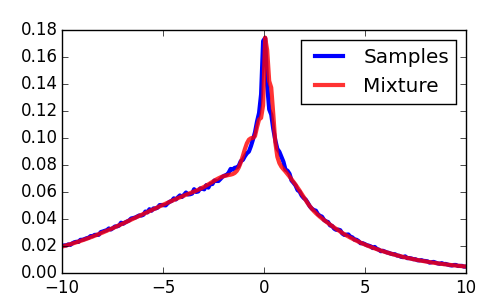
\includegraphics[width=\textwidth]{thesis/theory/gauss-hermite}
    \caption{An overview of the general fit}
    \label{fig:gauss-laguerre}
  \end{subfigure}
  \hfill
  \begin{subfigure}{0.45\textwidth}
    \centering
    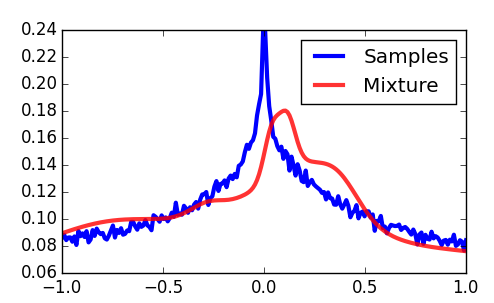
\includegraphics[width=\textwidth]{thesis/theory/gauss-hermite-zoomed}
    \caption{Zoomed in around $0$}
    \label{fig:gauss-laguerre-zoomed}
  \end{subfigure}
  \caption{A product distribution approximated by a mixture of Gaussians}
\end{figure}
Figure \ref{fig:gauss-laguerre} shows, that the calculated mixture of Gaussians
closely follows the true PDF obtained by sampling except in a neighborhood of
$0$. The zoomed-in plot in figure \ref{fig:gauss-laguerre-zoomed} confirms
indeed, that the approximation still has a similar shape, but is more wobbly
than the true PDF in the proximity of $0$.

The bad fit around $0$ is actually inherent to our problem and choice of
algorithm. Remember the requirement of any Gauss quadrature method, that $f$ be
in $C^{2n - 1}[a, b]$, and then look at the original integral and its integrand
as a function of $y$.
\begin{equation*}
  \int_{-\infty}^{\infty} \mathcal{N}\left( z \mid y\mu, y^{2}\sigma^{2} \right) \cdot \mathcal{N}(y \mid \nu, \tau^{2})~\mathrm{d}y
\end{equation*}
If $z = 0$ and $y$ approaches $0$, the integrand tends towards $\infty$ from
both sides, so it is not even once continuously differentiable in $0$, though it
is continuously differentiable infinite times everywhere else. So any Gauss
quadrature method will be numerically unstable. It is, however, sufficiently
stable for our cause, if you evaluate it with $z$ not too close $0$, which is
also evident in figure \ref{fig:gauss-laguerre}.

The problem obviously persists after the substitution, but now we can pinpoint
exactly, where the instabily will occur. Recall the transformed integral
\begin{equation*}
  \int_{-\infty}^{\infty} \mathcal{N}\left( z \mid \left(\sqrt{2}\tau x + \nu\right)\mu, \left(\sqrt{2}\tau x + \nu\right)^{2}\sigma^{2} \right) \cdot \exp\left( -x^{2} \right)~\mathrm{d}x
\end{equation*}
We have the same problem as before, when $\sqrt{2}\tau x + \nu$ is small,
i.e. $x \approx -\frac{\nu}{\sqrt{2}\tau}$, and
$z \approx \left(\sqrt{2}\tau x + \nu\right)\mu$. In figure
\ref{fig:gauss-hermite-instabilities} we plot the 10 components with minimal
variance. Their $x$-value is their mean and their $y$-value their variance. We
observe, that all of them are in direct proximity of the instability.
\begin{figure}[h]
  \centering
  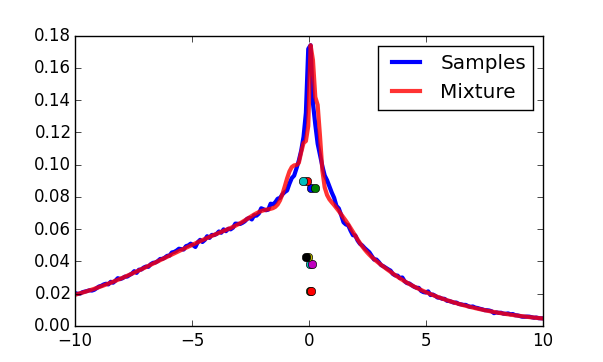
\includegraphics[width=0.6\textwidth]{thesis/theory/gauss-hermite-instabilities}
  \caption{The components with minimal variance are in direct proximity of the
    instability}
  \label{fig:gauss-hermite-instabilities}
\end{figure}

\subsubsection{Gauss-Laguerre Quadrature}

Another algorithm in the family of Gauss quadratures is Gauss-Laguerre
quadrature. It is made for integrals of the form
\begin{equation*}
  \int_{0}^{\infty} f(x) \cdot \exp(-x)~\mathrm{d}x
\end{equation*}
which does not match our situation quite as well as Gauss-Hermite does, so we
will need to do some more preparatory work. The motivation for trying
Gauss-Laguerre quadrature is, that this procedure may cope better with the
instability around $0$.

To make Gauss-Laguerre quadrature applicable, we have to rewrite the integral
from $-\infty$ to $\infty$ as two integrals from $0$ to $\infty$.
\begin{align*}
  p(Z = z) & = \int_{-\infty}^{\infty} \mathcal{N}\left( z \mid y\mu, y^{2}\sigma^{2} \right) \cdot \mathcal{N}(y \mid \nu, \tau^{2})~\mathrm{d}y\\
           & = \int_{-\infty}^{0} \mathcal{N}\left( z \mid y\mu, y^{2}\sigma^{2} \right) \cdot \mathcal{N}(y \mid \nu, \tau^{2})~\mathrm{d}y + \int_{0}^{\infty} \mathcal{N}\left( z \mid y\mu, y^{2}\sigma^{2} \right) \cdot \mathcal{N}(y \mid \nu, \tau^{2})~\mathrm{d}y\\
           & = -\int_{\infty}^{0} \mathcal{N}\left( z \mid -y\mu, y^{2}\sigma^{2} \right) \cdot \mathcal{N}(-y \mid \nu, \tau^{2})~\mathrm{d}y + \int_{0}^{\infty} \mathcal{N}\left( z \mid y\mu, y^{2}\sigma^{2} \right) \cdot \mathcal{N}(y \mid \nu, \tau^{2})~\mathrm{d}y\\
           & = \int_{0}^{\infty} \mathcal{N}\left( z \mid -y\mu, y^{2}\sigma^{2} \right) \cdot \mathcal{N}(-y \mid \nu, \tau^{2})~\mathrm{d}y + \int_{0}^{\infty} \mathcal{N}\left( z \mid y\mu, y^{2}\sigma^{2} \right) \cdot \mathcal{N}(y \mid \nu, \tau^{2})~\mathrm{d}y
\end{align*}

Both of these integrals can be solved approximately through Gauss-Laguerre
integration. Yet we will first have to rewrite them in the required form and
once again the integrands are not sufficiently differentiable in $0$. This time
we may be able to avert the problem though through a very non-mathematical
approach. Instead of integrating over $[0, \infty]$ we integrate over
$[\varepsilon, \infty]$ for an $\varepsilon > 0$. For some $\varepsilon$ the
payoff from not evaluating the integrand in the proximity of the instability may
be greater than the reduced accuracy from ignoring an $\varepsilon$-strip of the
integral.

We begin with rearranging the first integrand to the form $f(y) * e^{-y}$.
\begin{align*}
  & \int_{\varepsilon}^{\infty} \mathcal{N}\left( z \mid -y\mu, y^{2}\sigma^{2} \right) \cdot \mathcal{N}(-y \mid \nu, \tau^{2})~\mathrm{d}y \\
  =& \int_{\varepsilon}^{\infty} \mathcal{N}\left( z \mid -y\mu, y^{2}\sigma^{2} \right) \cdot \frac{1}{\sqrt{2 \pi \tau^{2}}} \exp\left( -\frac{(-y - \nu)^{2}}{2\tau^{2}} \right)~\mathrm{d}y\\
  =& \int_{\varepsilon}^{\infty} \mathcal{N}\left( z \mid -y\mu, y^{2}\sigma^{2} \right) \cdot \frac{1}{\sqrt{2 \pi \tau^{2}}} \exp\left( -\left( \frac{y + \nu}{\sqrt{2\tau^{2}}} \right)^{2} \right)~\mathrm{d}y\\
  \intertext{Substitute $t = \left( \frac{y + \nu}{\sqrt{2\tau^{2}}} \right)^{2}$, $y = \pm \sqrt{2\tau^{2} t} - \nu$, $\frac{\mathrm{d}t}{\mathrm{d}y} = \frac{y + \nu}{\tau^{2}} = \frac{(\pm \sqrt{2\tau^{2} t} - \nu) + \nu}{\tau^{2}} = \pm \frac{\sqrt{2t}}{\sqrt{\tau^{2}}}$}
  =& \int_{\frac{(\varepsilon + \nu)^{2}}{2\tau^{2}}}^{\infty} \mathcal{N}\left( z \mid -\left( \sqrt{2\tau^{2} t} - \nu \right)\mu, \left( \sqrt{2\tau^{2} t} - \nu \right)^{2}\sigma^{2} \right) \cdot \frac{1}{2 \sqrt{\pi t}} \exp\left( -t \right)~\mathrm{d}t\\
  \intertext{Substitute $s = t - \frac{(\varepsilon + \nu)^{2}}{2\tau^{2}}$, $t = s + \frac{(\varepsilon + \nu)^{2}}{2\tau^{2}}$, $\frac{\mathrm{d}s}{\mathrm{d}t} = 1$}
  =& \int_{0}^{\infty} \mathcal{N}\left( z \left| \ontopof{-\left( \sqrt{2\tau^{2}s + (\varepsilon + \nu)^{2}} - \nu \right)\mu}{\left( \sqrt{2\tau^{2}s + (\varepsilon + \nu)^{2}} - \nu \right)^{2}\sigma^{2}} \right.\right) \cdot \frac{\exp\left( -\frac{(\varepsilon + \nu)^{2}}{2\tau^{2}} \right)}{2 \sqrt{\pi \left( s + \frac{(\varepsilon + \nu)^{2}}{2\tau^{2}} \right)}} \exp(-s)~\mathrm{d}s
\end{align*}

Next we rearrange the second integrand.
\begin{align*}
  & \int_{\varepsilon}^{\infty} \mathcal{N}\left( z \mid y\mu, y^{2}\sigma^{2} \right) \cdot \mathcal{N}(y \mid \nu, \tau^{2})~\mathrm{d}y\\
  =& \int_{\varepsilon}^{\infty} \mathcal{N}\left( z \mid y\mu, y^{2}\sigma^{2} \right) \cdot \frac{1}{\sqrt{2 \pi \tau^{2}}} \exp\left( -\frac{(y - \nu)^{2}}{2\tau^{2}} \right)~\mathrm{d}y\\
  =& \int_{\varepsilon}^{\infty} \mathcal{N}\left( z \mid y\mu, y^{2}\sigma^{2} \right) \cdot \frac{1}{\sqrt{2 \pi \tau^{2}}} \exp\left( -\left( \frac{y - \nu}{\sqrt{2\tau^{2}}} \right)^{2} \right)~\mathrm{d}y\\
  \intertext{Substitute $t = \left( \frac{y - \nu}{\sqrt{2\tau^{2}}} \right)^{2}$, $y = \pm \sqrt{2\tau^{2} t} + \nu$, $\frac{\mathrm{d}t}{\mathrm{d}y} = \frac{y - \nu}{\tau^{2}} = \frac{(\pm \sqrt{2\tau^{2} t} + \nu) - \nu}{\tau^{2}} = \pm \frac{\sqrt{2t}}{\sqrt{\tau^{2}}}$}
  =& \int_{\frac{(\varepsilon - \nu)^{2}}{2\tau^{2}}}^{\infty} \mathcal{N}\left( z \mid \left( \sqrt{2\tau^{2} t} + \nu \right)\mu, \left( \sqrt{2\tau^{2} t} + \nu \right)^{2}\sigma^{2} \right) \cdot \frac{1}{2\sqrt{\pi t}} \exp\left( -t \right)~\mathrm{d}t\\
  \intertext{Substitute $s = t - \frac{(\varepsilon - \nu)^{2}}{2\tau^{2}}$, $t = s + \frac{(\varepsilon - \nu)^{2}}{2\tau^{2}}$, $\frac{\mathrm{d}s}{\mathrm{d}t} = 1$}
  =& \int_{0}^{\infty} \mathcal{N}\left( z \left| \ontopof{\left( \sqrt{2\tau^{2} s + (\varepsilon - \nu)^{2}} + \nu \right)\mu}{\left( \sqrt{2\tau^{2} s + (\varepsilon - \nu)^{2}} + \nu \right)^{2}\sigma^{2}} \right.\right) \cdot \frac{\exp\left( -\frac{(\varepsilon - \nu)^{2}}{2\tau^{2}} \right)}{2\sqrt{\pi \left( s + \frac{(\varepsilon - \nu)^{2}}{2\tau^{2}} \right)}} \exp(-s)~\mathrm{d}s
\end{align*}

Now we can plug in the two rearrangements and get the approximation as a mixture
of Gaussians by applying the Gauss-Laguerre quadrature.
\begin{align*}
  p(Z = z) \approx& \int_{0}^{\infty} \mathcal{N}\left( z \left| \ontopof{-\left( \sqrt{2\tau^{2}s + (\varepsilon + \nu)^{2}} - \nu \right)\mu}{\left( \sqrt{2\tau^{2}s + (\varepsilon + \nu)^{2}} - \nu \right)^{2}\sigma^{2}} \right.\right) \cdot \frac{\exp\left( -\frac{(\varepsilon + \nu)^{2}}{2\tau^{2}} \right)}{2 \sqrt{\pi \left( s + \frac{(\varepsilon + \nu)^{2}}{2\tau^{2}} \right)}} \exp(-s)~\mathrm{d}s\\
                  & + \int_{0}^{\infty} \mathcal{N}\left( z \left| \ontopof{\left( \sqrt{2\tau^{2} s + (\varepsilon - \nu)^{2}} + \nu \right)\mu}{\left( \sqrt{2\tau^{2} s + (\varepsilon - \nu)^{2}} + \nu \right)^{2}\sigma^{2}} \right.\right) \cdot \frac{\exp\left( -\frac{(\varepsilon - \nu)^{2}}{2\tau^{2}} \right)}{2\sqrt{\pi \left( s + \frac{(\varepsilon - \nu)^{2}}{2\tau^{2}} \right)}} \exp(-s)~\mathrm{d}s\\
  \approx& \sum_{i = 1}^{n} w_{i} \frac{\exp\left( -\frac{(\varepsilon + \nu)^{2}}{2\tau^{2}} \right)}{2 \sqrt{\pi \left( x_{i} + \frac{(\varepsilon + \nu)^{2}}{2\tau^{2}} \right)}} \cdot \mathcal{N}\left( z \left|
           \ontopof{-\left( \sqrt{2\tau^{2}x_{i} + (\varepsilon + \nu)^{2}} - \nu \right)\mu}{\left( \sqrt{2\tau^{2}x_{i} + (\varepsilon + \nu)^{2}} - \nu \right)^{2}\sigma^{2}}
           \right.\right)\\
                  &+ \sum_{i = 1}^{n} w_{i} \frac{\exp\left( -\frac{(\varepsilon - \nu)^{2}}{2\tau^{2}} \right)}{2\sqrt{\pi \left( x_{i} + \frac{(\varepsilon - \nu)^{2}}{2\tau^{2}} \right)}} \cdot \mathcal{N}\left( z \left|
                    \ontopof{\left( \sqrt{2\tau^{2} x_{i} + (\varepsilon - \nu)^{2}} + \nu \right)\mu}{\left( \sqrt{2\tau^{2} x_{i} + (\varepsilon - \nu)^{2}} + \nu \right)^{2}\sigma^{2}}
                    \right.\right)
\end{align*}
where the $x_{i}$ are the roots of the $n$-th Laguerre polynomial and the
$w_{i}$ the associated weights.

This time things did not turn out as nice as with Gauss-Hermite quadrature. The
$\sum_{i} w_{i}$ is $1$ and the value of the coefficients is overall not
constant, so the sums are not a real mixture distribution and the weights have
to be normalized. This method also cannot keep up in a direct comparison (figure
\ref{fig:hermite-laguerre}). Both methods find the correct mean and
Gauss-Laguerre quadrature also produces a shape similar to the true probability
density, but apart from that it is pretty far off. The variance in the proximity
of the instability is too small, but overall it is too high. In this example the
sample variance is roughly $40$, closely matched by the Gauss-Hermite
approximation, but the variance of the Gauss-Laguerre mixture is $80$. There may
be a bug in our program or an error in the math of this section regarding the
variance, though we did not find any.
\begin{figure}[h]
  \centering
  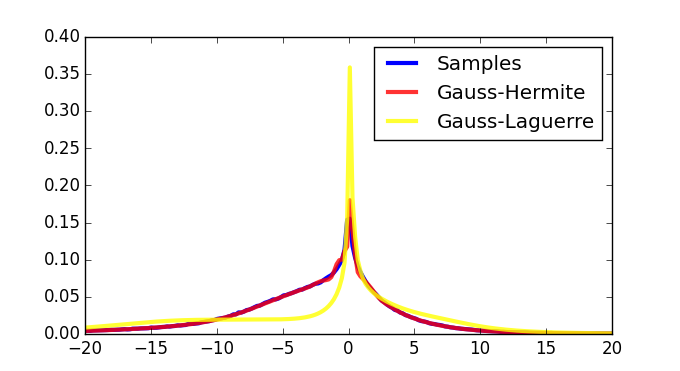
\includegraphics[width=0.65\textwidth]{thesis/theory/hermite-laguerre}
  \caption{Gauss-Laguerre cannot keep up with Gauss-Hermite}
  \label{fig:hermite-laguerre}
\end{figure}

\subsection{Quotients of Gaussian Random Variables}

Division shares all the important properties with multiplication: It, too, is
differentiable and monotonic in the first argument and Gaussian distributions
are not closed under it. So we have to use numerical approximation again. This
time we only try Gauss-Hermite quadrature, because the integrand has a very
similar form and it served us well for multiplication.

Let $X$ and $Y$ be two normally distributed variables
\begin{equation*}
  X \sim \mathcal{N}(\mu, \sigma^{2}) \qquad Y \sim \mathcal{N}(\nu, \tau^{2})
\end{equation*}
and $Z = \frac{X}{Y}$ their quotient. Then $Z$ is distributed as follows
\begin{align*}
  p(Z = z) & = \int_{-\infty}^{\infty} |y| \cdot p\left(X = zy\right) \cdot p(Y = y)~\mathrm{d}y\\
           & = \int_{-\infty}^{\infty} |y| \cdot \mathcal{N}\left( zy \mid \mu, \sigma^{2} \right) \cdot \mathcal{N}(y \mid \nu, \tau^{2})~\mathrm{d}y\\
           & = \int_{-\infty}^{\infty} |y| \cdot \frac{1}{|y|} \cdot \mathcal{N}\left( z \mid \frac{\mu}{y}, \frac{\sigma^{2}}{y^{2}} \right) \cdot \mathcal{N}(y \mid \nu, \tau^{2})~\mathrm{d}y\\
           & = \int_{-\infty}^{\infty} \mathcal{N}\left( z \mid \frac{\mu}{y}, \frac{\sigma^{2}}{y^{2}} \right) \cdot \mathcal{N}(y \mid \nu, \tau^{2})~\mathrm{d}y
\end{align*}
Now we can apply the same substitution as in the multiplication case to bring it
into Gauss-Hermite quadrature form and get
\begin{equation*}
  p(Z = z) \approx \sum_{i = 1}^{n} \frac{w_{i}}{\sqrt{\pi}} \cdot \mathcal{N}\left( z \left| \frac{\mu}{\sqrt{2 \tau^{2}} x_{i} + \nu}, \frac{\sigma^{2}}{\left(\sqrt{2 \tau^{2}} x_{i} + \nu\right)^{2}} \right.\right)
\end{equation*}

Figure \ref{fig:hermite-division} shows, that the fit is even better this time
and there are no instabilities around~$0$. This is surprising, if you consider
the problems we had with approximating a product distribution.
\begin{figure}[h]
  \centering
  \begin{subfigure}{0.45\textwidth}
    \centering
    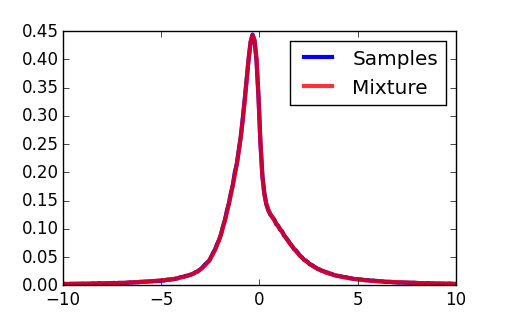
\includegraphics[width=\textwidth]{thesis/theory/division}
    \caption{Overview}
  \end{subfigure}
  \hfill
  \begin{subfigure}{0.45\textwidth}
    \centering
    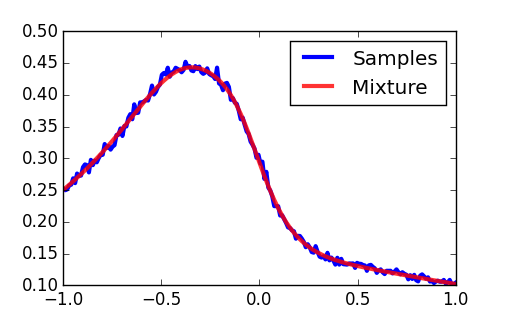
\includegraphics[width=\textwidth]{thesis/theory/division-zoomed}
    \caption{Zoomed in around $0$}
  \end{subfigure}
  \caption{Gauss-Hermite approximates a ratio distribution perfectly}
  \label{fig:hermite-division}
\end{figure}

The explanation is, that in this case the integrand is actually in
$C^{\infty}[-\infty, \infty]$, because you can eliminate $y$ from all
denominators.
\begin{align*}
  \mathcal{N}\left( z \mid \frac{\mu}{y}, \frac{\sigma^{2}}{y^{2}} \right) \cdot \mathcal{N}(y \mid \nu, \tau^{2}) = & \frac{1}{\sqrt{2 \pi \frac{\sigma^{2}}{y^{2}}}} \exp\left( -\frac{\left( z - \frac{\mu}{y} \right)^{2}}{2\frac{\sigma^{2}}{y^{2}}} \right) \cdot \frac{1}{\sqrt{2 \pi \tau^{2}}} \exp\left( -\frac{(y - \nu)^{2}}{2\tau^{2}} \right)\\
  = & \frac{y}{2\pi\sigma\tau} \cdot \exp\left( -\frac{\frac{1}{y^{2}}\left( zy - \mu \right)^{2}y^{2}}{2\sigma^{2}} \right) \cdot \exp\left( -\frac{(y - \nu)^{2}}{2\tau^{2}} \right)\\
  = & \frac{y}{2\pi\sigma\tau} \cdot \exp\left( -\frac{\left( zy - \mu \right)^{2}}{2\sigma^{2}} \right) \cdot \exp\left( -\frac{(y - \nu)^{2}}{2\tau^{2}} \right)\\
\end{align*}
So the exponents are just polynomials. Since polynomials, compositions and
products of functions in $C^{\infty}$ are in turn in $C^{\infty}$, the whole
integrand is in $C^{\infty}$.

\chapter{Implementation}
\label{ch:implementation}

The accompanying implementation is written in julia \cite{julia}, a new
programming language for technical computing. It was originally developed by a
group of four applied mathematicians at MIT and has since amassed a significant
following in the applied mathematics and data science communities.

The foundation of the implementation is a library called Distributions.jl
\cite{distributionsjl}, that defines types for all well-known distributions and
some exotic ones. A minor role plays StatsBase.jl \cite{statsbasejl} in our
implementation of EM, where it approximates the mean and variance of a
distribution from samples. Finally we depend on GaussQuadrature.jl \cite{gq} as
well as FastGaussQuadrature.jl \cite{fastgq} for computing the weights and
integration points for Gauss-Laguerre respectively Gauss-Hermite quadrature.

The central structure in the implementation is a type called
\injulia{RandomVariable}, that attaches parameters for the different integration
algorithms to a mixture distribution from Distributions.jl. The parameters
themselves are wrapped in a type per algorithm. The rest of the library is
pretty much just chapter \ref{ch:theory} translated from math to julia.

Notable is julia's multiple dispatch system, which allows us to integrate the
\injulia{RandomVariable} type seamlessly into julia's number system, so that you
can pass a \injulia{RandomVariable} everywhere you could pass a number as long
as you only use the supported operations.

The source code is attached in appendix \ref{ch:source} as well as published on
github \cite{github}.

\chapter{Demos}
\label{ch:comparisons}

In this chapter we will present example plots for all operations, that we have
examined, and combinations of them.

\section{Modelling with EM}

In section \ref{sec:em} we described, how to model arbitrary distributions as a
mixture of Gaussians. It would be interesting to see, how well this method
performs on various distributions and how many components you need, to get a
reasonable fit.

We observe, that there are two classes in regards to how well they can be
approximated by a mixture of Gaussians. The first group contains the symmetric
distributions with support $\mathbb{R}$. Examples are student's T (figure
\ref{fig:em-students-t}), Cauchy (figure \ref{fig:em-cauchy}) and Laplace
distributions (figure \ref{fig:em-laplace}).

\begin{figure}[h]
  \centering
  \begin{subfigure}{0.45\textwidth}
    \centering
    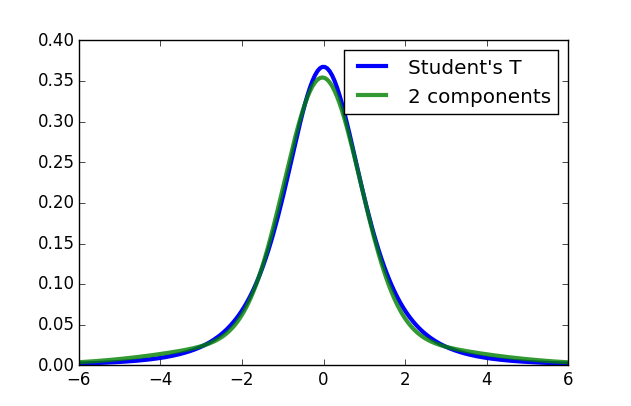
\includegraphics[width=\textwidth]{thesis/em/t-2-components}
  \end{subfigure}
  \hfill
  \begin{subfigure}{0.45\textwidth}
    \centering
    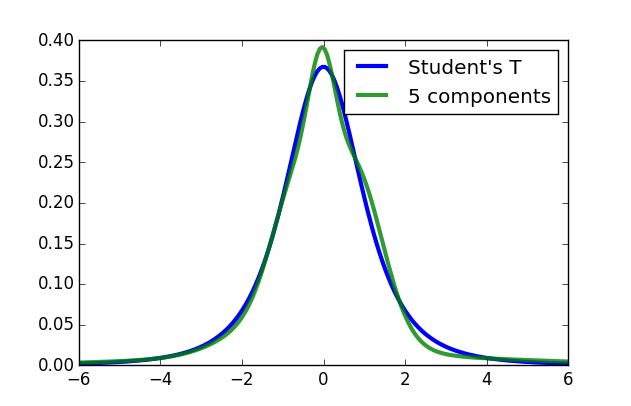
\includegraphics[width=\textwidth]{thesis/em/t-5-components}
  \end{subfigure}
  \caption{A student's T distribution is well approximated with a handful of
    components}
  \label{fig:em-students-t}
\end{figure}
\begin{figure}[h]
  \centering
  \begin{subfigure}{0.45\textwidth}
    \centering
    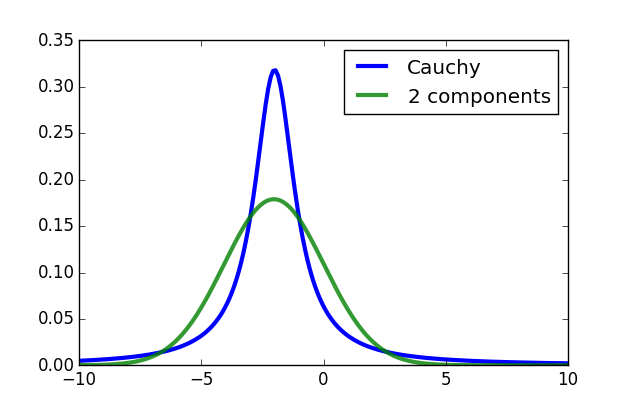
\includegraphics[width=\textwidth]{thesis/em/cauchy-2-components}
  \end{subfigure}
  \hfill
  \begin{subfigure}{0.45\textwidth}
    \centering
    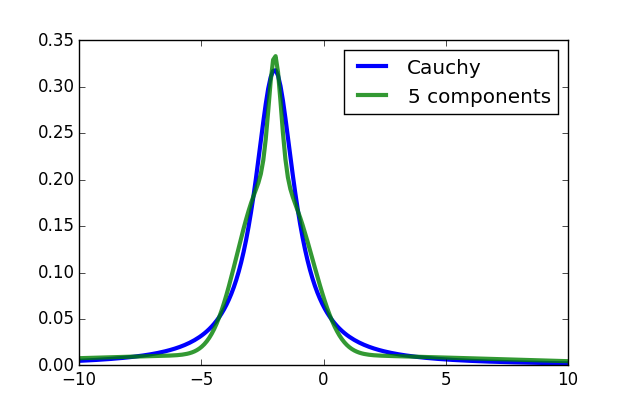
\includegraphics[width=\textwidth]{thesis/em/cauchy-5-components}
  \end{subfigure}
  \caption{A Cauchy distribution needs a few more components for a good fit}
  \label{fig:em-cauchy}
\end{figure}
\begin{figure}[h]
  \centering
  \begin{subfigure}{0.45\textwidth}
    \centering
    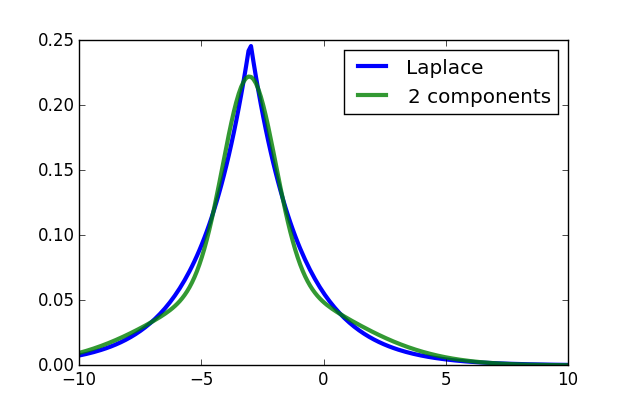
\includegraphics[width=\textwidth]{thesis/em/laplace-2-components}
  \end{subfigure}
  \hfill
  \begin{subfigure}{0.45\textwidth}
    \centering
    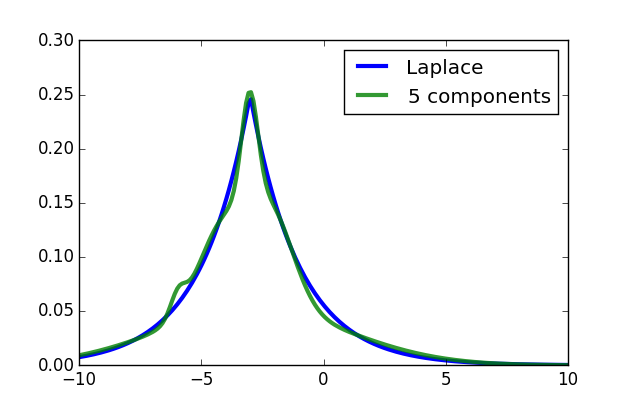
\includegraphics[width=\textwidth]{thesis/em/laplace-5-components}
  \end{subfigure}
  \caption{Two components are too few to recreate the peak of a Laplace
    distribution}
  \label{fig:em-laplace}
\end{figure}
All of these are very closely matched by a mixture of Gaussians with just $5$
components, but for some distributions even $2$ yield reasonable results.

The second class consists of the distributions, that are only defined on parts
of $\mathbb{R}$. Some of them are defined on $\mathbb{R}_{\ge 0}$, for example
the Gamma (figure \ref{fig:em-gamma}) or Weibull distributions (figure
\ref{fig:em-weibull}).
\begin{figure}[h]
  \centering
  \begin{subfigure}{0.45\textwidth}
    \centering
    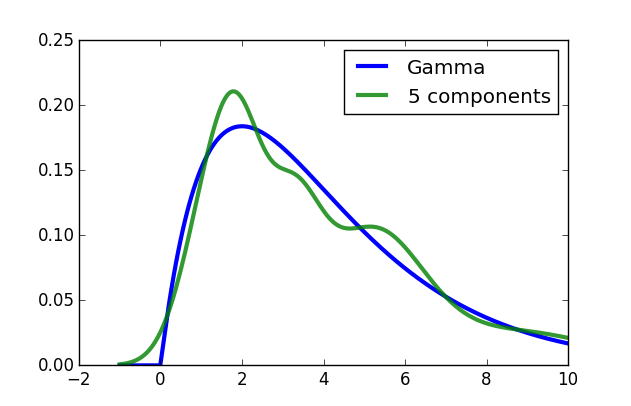
\includegraphics[width=\textwidth]{thesis/em/gamma-5-components}
  \end{subfigure}
  \hfill
  \begin{subfigure}{0.45\textwidth}
    \centering
    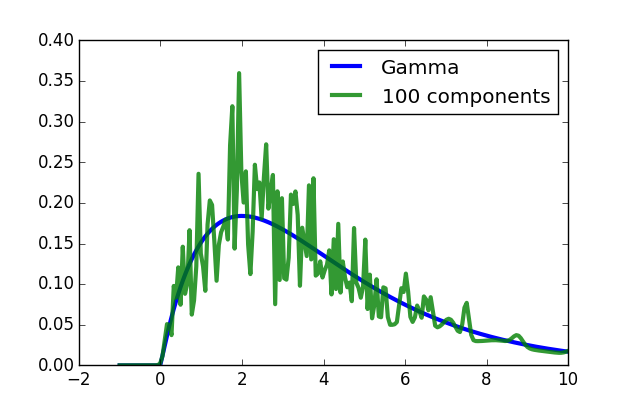
\includegraphics[width=\textwidth]{thesis/em/gamma-100-components}
  \end{subfigure}
  \caption{You can have few smooth components or a good fit at the corner}
  \label{fig:em-gamma}
\end{figure}
\begin{figure}[h]
  \centering
  \begin{subfigure}{0.45\textwidth}
    \centering
    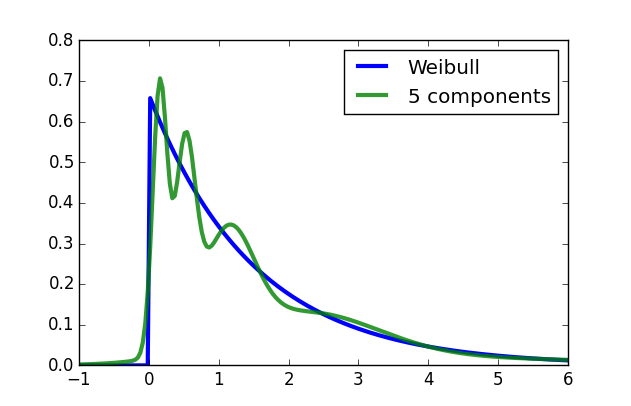
\includegraphics[width=\textwidth]{thesis/em/weibull-5-components}
  \end{subfigure}
  \hfill
  \begin{subfigure}{0.45\textwidth}
    \centering
    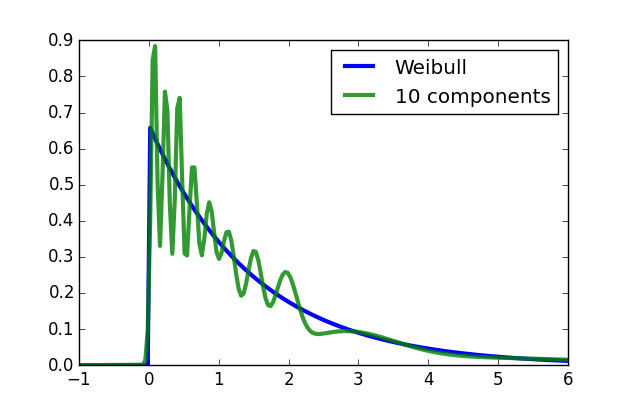
\includegraphics[width=\textwidth]{thesis/em/weibull-10-components}
  \end{subfigure}
  \caption{Recreating a $90^{\circ}$ corner is easier}
  \label{fig:em-weibull}
\end{figure}

Others are only defined on a finite interval, for instance a triangular (figure
\ref{fig:em-triangular}) or a uniform distribution (figure
\ref{fig:em-uniform}).

\begin{figure}[h]
  \centering
  \begin{subfigure}{0.45\textwidth}
    \centering
    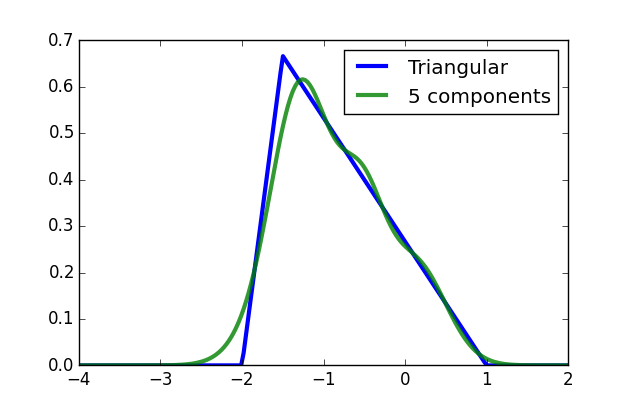
\includegraphics[width=\textwidth]{thesis/em/triangular-5-components}
  \end{subfigure}
  \hfill
  \begin{subfigure}{0.45\textwidth}
    \centering
    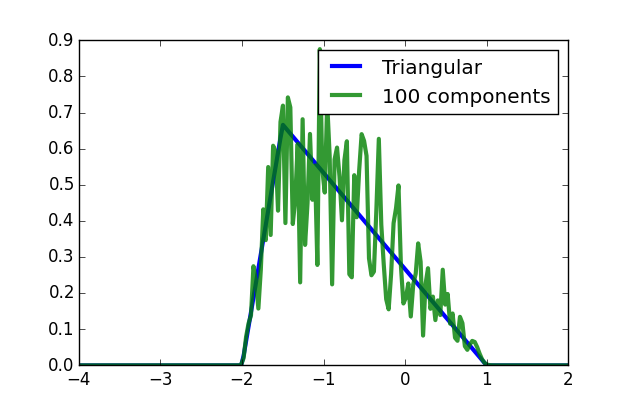
\includegraphics[width=\textwidth]{thesis/em/triangular-100-components}
  \end{subfigure}
  \caption{Double the corners, double the problems}
  \label{fig:em-triangular}
\end{figure}
\begin{figure}[h]
  \centering
  \begin{subfigure}{0.45\textwidth}
    \centering
    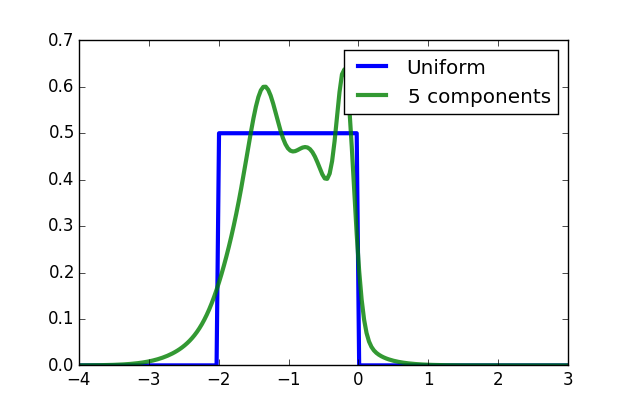
\includegraphics[width=\textwidth]{thesis/em/uniform-5-components}
  \end{subfigure}
  \hfill
  \begin{subfigure}{0.45\textwidth}
    \centering
    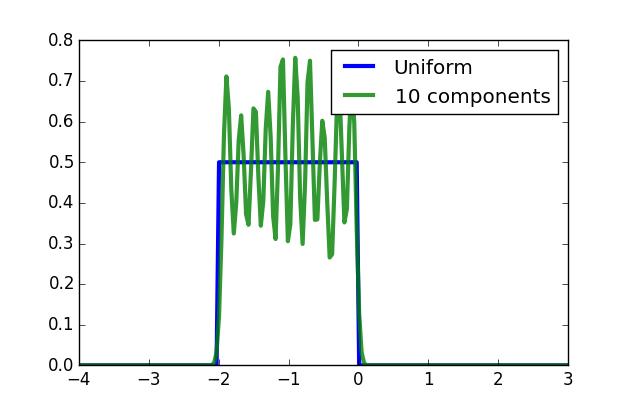
\includegraphics[width=\textwidth]{thesis/em/uniform-10-components}
  \end{subfigure}
  \caption{Modelling a uniform distribution works surprisingly well}
  \label{fig:em-uniform}
\end{figure}

Yet they all share the property, that they have corners, points where the
probability density more or less abruptly becomes $0$. Modelling these points is
hard. There is a trade-off between the number of components and the smoothness
of the approximation. You may get a reasonable approximation with a handful of
components, but it will not model the corner very well, because the few
components will have to be broad and smooth to model the bulk of the probability
mass. The corners may be very important though. If your random variable is Gamma
distributed, you really do not want any probability mass in
$\mathbb{R}_{\le 0}$. And a high number of components will accomplish that. It
will, however, also make the approximation a lot less smooth, because the corner
has to be modelled by approaching it with progressively more peaked components.

An interesting observation is, that you need less components to model a
$90^{\circ}$ corner than if it were of another degree.

\section{Operations on Mixtures of Gaussians}

Next we examined arithmetic operations on mixtures of Gaussians, which we will
showcase in this section.

\subsection{Affine Transformations}

Affine transformations are less interesting in the context of this thesis,
because they can be calculated exactly through parameter transformations. We
will plot one anyway to demonstrate, that the attached library can correctly
compute it. In figure \ref{fig:affine} we apply the affine transformation
\begin{equation*}
  f(a, b, c) = \frac{3a}{5} + 2b - c - 3
\end{equation*}
to the variables plotted in figure \label{fig:affine-vars}. The computed mixture
plotted in figure \ref{fig:affine-result} is congruent to the sampled PDF as
expected.
\begin{figure}[h]
  \centering
  \begin{subfigure}[t]{0.45\textwidth}
    \centering
    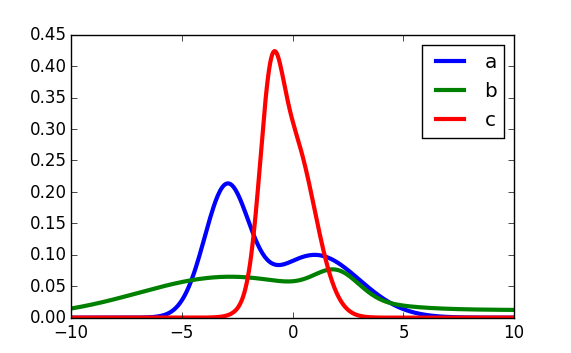
\includegraphics[width=\textwidth]{thesis/operations/affine-vars}
    \caption{The variables to transform}
    \label{fig:affine-vars}
  \end{subfigure}
  \hfill
  \begin{subfigure}[t]{0.45\textwidth}
    \centering
    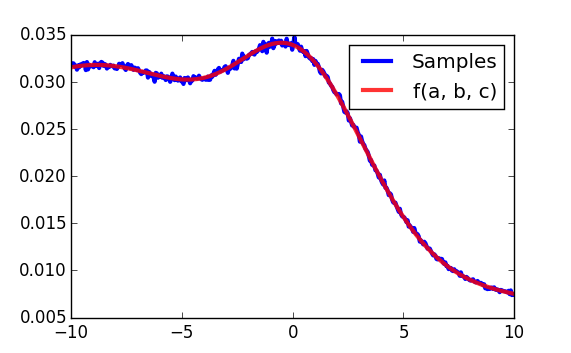
\includegraphics[width=\textwidth]{thesis/operations/affine-result}
    \caption{The resulting density on top of the sampled density}
    \label{fig:affine-result}
  \end{subfigure}
  \caption{Affine transformations are calculated exactly}
  \label{fig:affine}
\end{figure}

\subsection{Products with Gauss-Hermite}

\begin{figure}[h]
  \centering
  \begin{subfigure}[t]{0.45\textwidth}
    \centering
    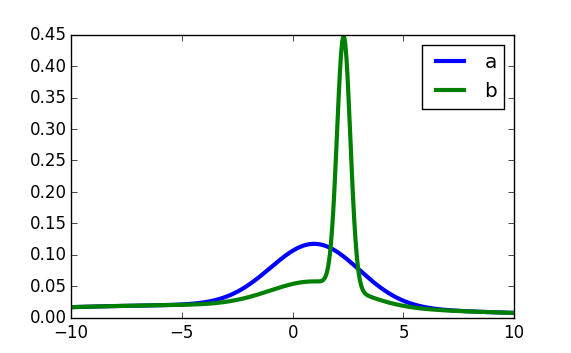
\includegraphics[width=\textwidth]{thesis/operations/product-hermite-vars}
    \caption{The variables to multiply}
    \label{fig:product-hermite-vars}
  \end{subfigure}
  \hfill
  \begin{subfigure}[t]{0.45\textwidth}
    \centering
    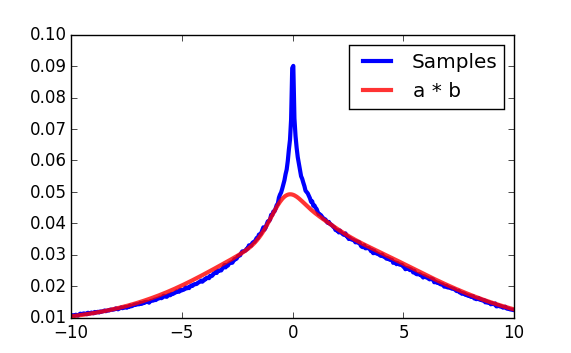
\includegraphics[width=\textwidth]{thesis/operations/product-hermite-50-components}
    \caption{Approximating the product distribution with $300$ components}
  \end{subfigure}
  \caption{Approximating a product distribution}
  \label{fig:product-hermite}
\end{figure}
\begin{figure}[h]
  \centering
  \begin{subfigure}[t]{0.45\textwidth}
    \centering
    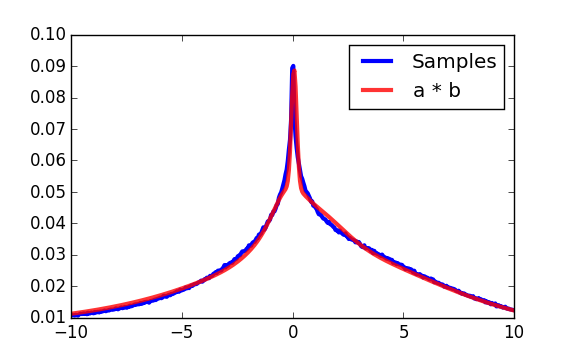
\includegraphics[width=\textwidth]{thesis/operations/product-hermite-100-components}
    \caption{600 components}
    \label{fig:product-hermite-vars}
  \end{subfigure}
  \hfill
  \begin{subfigure}[t]{0.45\textwidth}
    \centering
    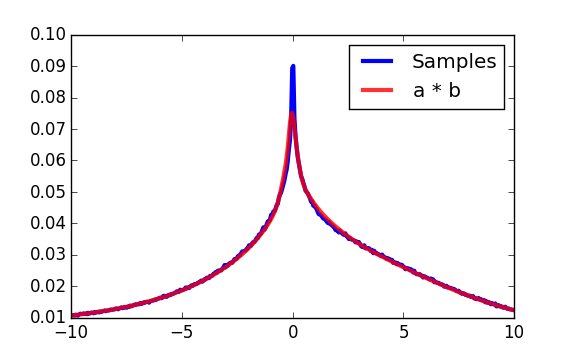
\includegraphics[width=\textwidth]{thesis/operations/product-hermite-2000-components}
    \caption{12000 components}
  \end{subfigure}
  \caption{You really need a lot of components to model it near the instability}
  \label{fig:product-hermite-2}
\end{figure}

\subsection{Products with Gauss-Laguerre}

\begin{figure}[h]
  \centering
  \begin{subfigure}[t]{0.45\textwidth}
    \centering
    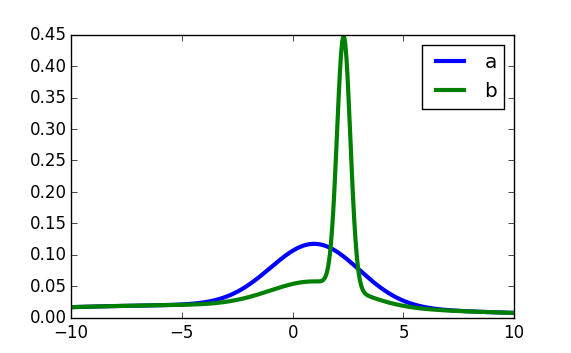
\includegraphics[width=\textwidth]{thesis/operations/product-laguerre-vars}
    \caption{The variables to multiply}
  \end{subfigure}
  \hfill
  \begin{subfigure}[t]{0.45\textwidth}
    \centering
    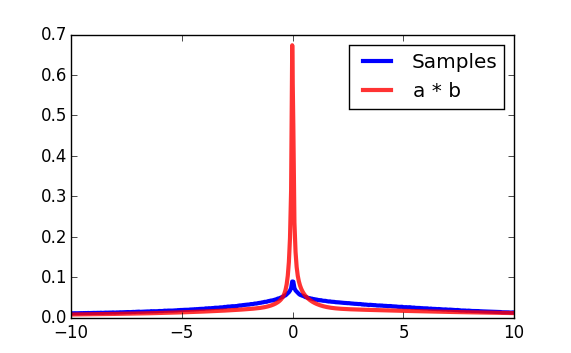
\includegraphics[width=\textwidth]{thesis/operations/product-laguerre-0}
    \caption{Approximation with $\varepsilon = 0$}
  \end{subfigure}
  \caption{Gauss-Laguerre produces pretty bad results}
  \label{fig:product-laguerre}
\end{figure}
\begin{figure}[h]
  \centering
  \begin{subfigure}[t]{0.45\textwidth}
    \centering
    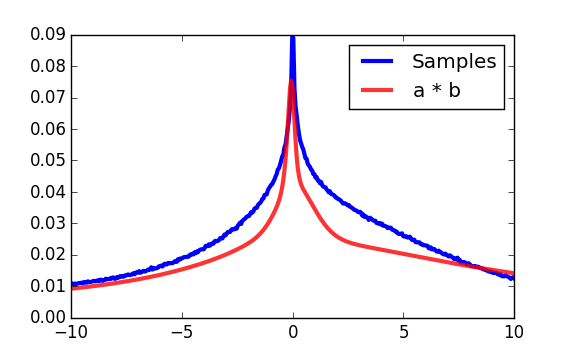
\includegraphics[width=\textwidth]{thesis/operations/product-laguerre-5}
    \caption{Approximation with $\varepsilon = 0.05$}
  \end{subfigure}
  \hfill
  \begin{subfigure}[t]{0.45\textwidth}
    \centering
    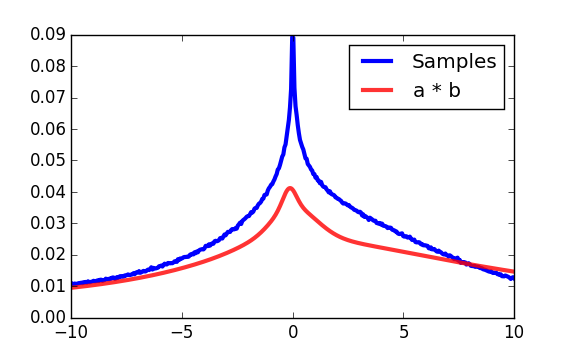
\includegraphics[width=\textwidth]{thesis/operations/product-laguerre-10}
    \caption{Approximation with $\varepsilon = 0.1$}
  \end{subfigure}
  \caption{At least the idea works, that you can control the height of the peaks
    through $\varepsilon$}
  \label{fig:product-laguerre}
\end{figure}

\subsection{Quotients}

\begin{figure}[h]
  \centering
  \begin{subfigure}[t]{0.45\textwidth}
    \centering
    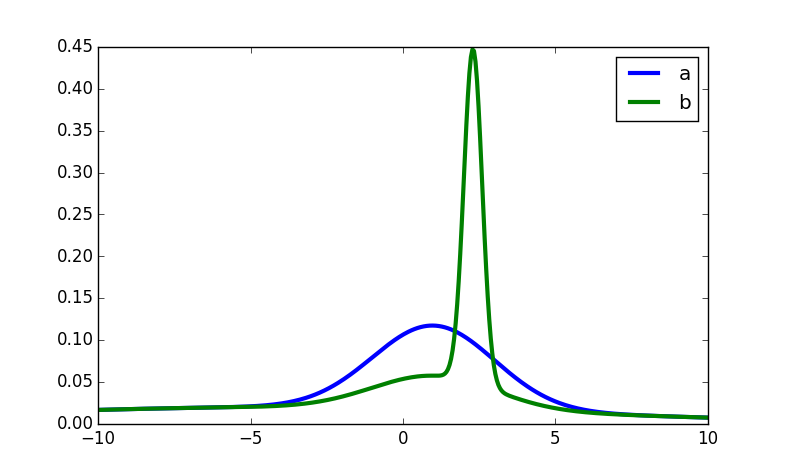
\includegraphics[width=\textwidth]{thesis/operations/quotient-vars}
    \caption{The variables to divide}
  \end{subfigure}
  \hfill
  \begin{subfigure}[t]{0.45\textwidth}
    \centering
    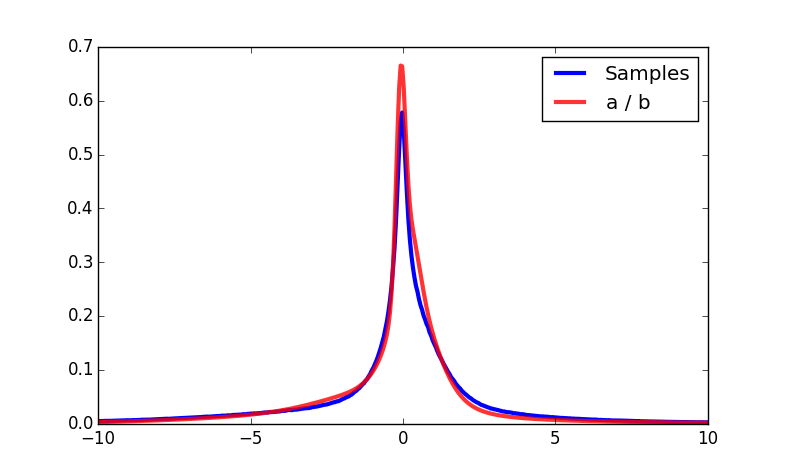
\includegraphics[width=\textwidth]{thesis/operations/quotient-2-components}
    \caption{Approximation with $12$ components}
  \end{subfigure}
  \caption{Just $12$ components give you are good fit already}
  \label{fig:quotient}
\end{figure}

\section{Complex Examples}

\chapter{Conclusions and Further Work}
\label{ch:conclusions}

We have shown, that the way of symbolic approximation works and yields results
comparable to ones derived through sampling or symbolic manipulation. It has to
be said though, that the scope of this project is currently limited. To really
keep up with the competing techniques, mixture approximation needs improvements
in several areas ranging from easy to hard.

The first and obvious improvement would be to implement more operations. At the
moment we are limited to basic arithmetic, but there surely are more functions,
that are differentiable and monotonic in the first argument. A related idea is
the implementation of a fallback algorithm for unimplemented operations. A naive
approach is to fall back on sampling and sample from the inputs, apply the
operation and then fit a new mixture to the samples with EM. But maybe there is
another way, that uses the fact, that everything is mixture distributed, more
directly and avoids the involvment of sampling.

An orthogonal idea is the use of other component distributions, which we already
hinted at throughout section \ref{sec:closure}. The problem with Gaussian
components is, that the math only allows to apply functions, that are defined on
at least the complete support of the inputs. This forbids things like taking the
logarithm of a mixture of Gaussians, because they will always have non-zero
probability of being negative no matter what the means and variances are. Gamma
and inverse Gaussian distributions are promising candidates, that only allow
positive reals, but at the same time have two parameters to influence mean and
variance and may thus give similar flexibility as a mixture of Gaussians.

Presumably rather easy would be the generalization to
$f : \mathbb{R}^{n} \rightarrow \mathbb{R}^{m}$, i.e. allow $f$ to have multiple
outputs.

From a performance point of view it would be useful to put a bound on the number
of components, that a mixture can have. Maybe there is a way to cut components
from a mixture and amend the remaining components' parameters, such that the
additional error from this operation is controllable and bounded. In the current
implementation the product and quotient of two Gaussian variables are
approximated by a mixture with $n$ components if you are evaluating it with
Gauss-Hermite at $n$ integration points. This means, that the product of three
mixtures with $a$, $b$ and $c$ components results in a mixture with $abcn^{2}$
components, which a huge number since $n$ is normally in the low hundreds.

The hardest part with the biggest payoff at the same time would be extending our
techniques to dependent variables. You would have to redo almost everything in
much more complex, because lemma \ref{lemma:mixture} does not hold for dependent
variables. The upside is, that you will be able to evaluate, for example, the
square of a random variable and generally terms with variables that are
dependent on each other in non-trivial ways.

\begin{appendices}
  \chapter{Source Code}
  \label{ch:source}

  \inputminted{julia}{src/Transforms.jl}
\end{appendices}

\printbibliography

\pagestyle{empty}
\cleardoublepage

\vspace*{10em}
{\LARGE Ehrenwörtliche Erklärung}
\vspace{1em}

Hiermit versichere ich, dass ich die Bachelorarbeit selbstständig und ohne
Benutzung anderer als der angegebenen Hilfsmittel verfasst und alle Stellen, die
wörtlich oder sinngemäß aus veröffentlichten Schriften entnommen sind, als
solche kenntlich gemacht habe.

\vspace{5em}

\begin{minipage}{0.4\textwidth}
  \begin{flushleft}
    Düsseldorf, 15. Juli 2015
  \end{flushleft}
\end{minipage}
\hfill
\begin{minipage}{0.4\textwidth}
  \begin{flushright}
    Marten Lienen
  \end{flushright}
\end{minipage}

\end{document}